% plots_mom.tex
%
% Standalone TikZ/pgfplots document that produces plots_mom.pdf when
% compiled with pdflatex. The same bar charts are also embedded inline
% in main.tex (Section 5); this standalone version exists so that the
% PDF can be referenced as a separate artefact (and so that the figure
% can be re-typeset without re-compiling the entire report).
%
% Compile:
%   pdflatex plots_mom.tex
%
% A Python equivalent that reads benchmark_results.csv and produces
% the same figure with Matplotlib is available as
% plot_speed_vs_mom.py.

\documentclass[border=8pt]{standalone}
\usepackage{tikz}
\usepackage{pgfplots}
\pgfplotsset{compat=1.18}

\begin{document}
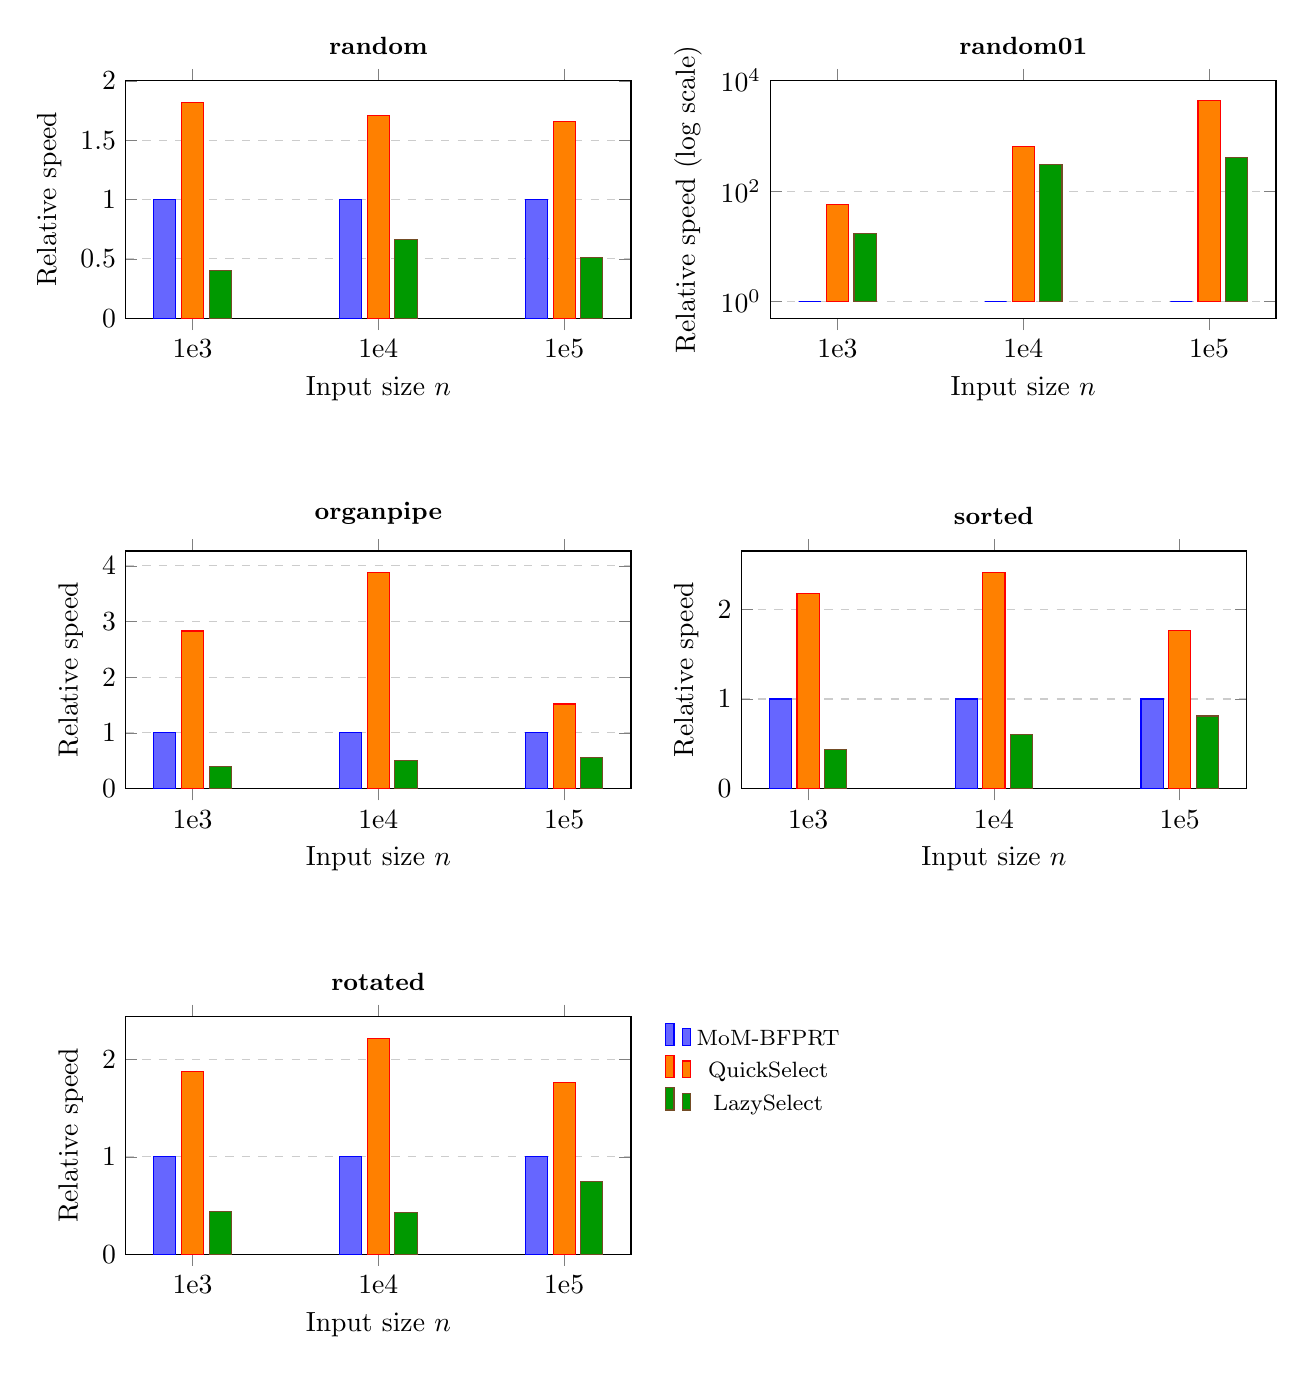
\begin{tikzpicture}

% Reusable style.
\pgfplotsset{
  panel/.style={
    ybar, width=8cm, height=4.6cm,
    enlarge x limits=0.18,
    legend style={at={(0.5,-0.30)}, anchor=north, legend columns=-1,
                  draw=none, font=\footnotesize},
    ylabel={Relative speed},
    xlabel={Input size $n$},
    symbolic x coords={1e3,1e4,1e5},
    xtick=data,
    bar width=8pt,
    ymajorgrids, grid style={dashed,gray!40},
    title style={font=\small\bfseries},
  }
}

% ---- Row 1: random / random01 -----------------------------------
\begin{axis}[panel, name=p1, title={random}, ymin=0]
  \addplot+[fill=blue!60]        coordinates {(1e3,1.00) (1e4,1.00) (1e5,1.00)};
  \addplot+[fill=orange]         coordinates {(1e3,1.82) (1e4,1.71) (1e5,1.66)};
  \addplot+[fill=green!60!black] coordinates {(1e3,0.40) (1e4,0.66) (1e5,0.51)};
\end{axis}

\begin{semilogyaxis}[
    ybar, width=8cm, height=4.6cm,
    enlarge x limits=0.18,
    ymin=0.5, ymax=10000,
    ylabel={Relative speed (log scale)},
    xlabel={Input size $n$},
    symbolic x coords={1e3,1e4,1e5},
    xtick=data,
    bar width=8pt,
    ymajorgrids, grid style={dashed,gray!40},
    title={random01}, title style={font=\small\bfseries},
    name=p2, at=(p1.right of east), anchor=left of west, xshift=12pt,
  ]
  \addplot+[fill=blue!60]        coordinates {(1e3,1.00)    (1e4,1.00)    (1e5,1.00)};
  \addplot+[fill=orange]         coordinates {(1e3,56.86)   (1e4,644.33)  (1e5,4364.18)};
  \addplot+[fill=green!60!black] coordinates {(1e3,17.30)   (1e4,303.53)  (1e5,404.06)};
\end{semilogyaxis}

% ---- Row 2: organpipe / sorted ----------------------------------
\begin{axis}[panel, title={organpipe}, ymin=0,
             at=(p1.below south west), anchor=above north west, yshift=-30pt,
             name=p3]
  \addplot+[fill=blue!60]        coordinates {(1e3,1.00) (1e4,1.00) (1e5,1.00)};
  \addplot+[fill=orange]         coordinates {(1e3,2.83) (1e4,3.88) (1e5,1.52)};
  \addplot+[fill=green!60!black] coordinates {(1e3,0.39) (1e4,0.50) (1e5,0.56)};
\end{axis}

\begin{axis}[panel, title={sorted}, ymin=0,
             at=(p3.right of east), anchor=left of west, xshift=12pt,
             name=p4]
  \addplot+[fill=blue!60]        coordinates {(1e3,1.00) (1e4,1.00) (1e5,1.00)};
  \addplot+[fill=orange]         coordinates {(1e3,2.18) (1e4,2.41) (1e5,1.76)};
  \addplot+[fill=green!60!black] coordinates {(1e3,0.44) (1e4,0.60) (1e5,0.81)};
\end{axis}

% ---- Row 3: rotated + legend ------------------------------------
\begin{axis}[panel, title={rotated}, ymin=0,
             legend style={at={(1.05,1.00)},anchor=north west,draw=none,
                            font=\footnotesize, legend columns=1},
             at=(p3.below south west), anchor=above north west, yshift=-30pt,
             name=p5]
  \addplot+[fill=blue!60]        coordinates {(1e3,1.00) (1e4,1.00) (1e5,1.00)};
  \addplot+[fill=orange]         coordinates {(1e3,1.88) (1e4,2.22) (1e5,1.76)};
  \addplot+[fill=green!60!black] coordinates {(1e3,0.44) (1e4,0.43) (1e5,0.75)};
  \legend{MoM-BFPRT, QuickSelect, LazySelect}
\end{axis}

\end{tikzpicture}
\end{document}
